%============================================================ 6. 결과 (압축판)
%  지휘관(LLM) 계층은 본 연구의 기여가 아니라 사용한 구성요소이므로, §6.2 는 표 두 개로
%  줄이고 도판을 두지 않는다. 도판은 기동 계층·체계 전체의 주장에만 쓴다.
\section{결과}
\label{sec:results}

\subsection{기동 계층의 기여}
\label{sec:res_g1}

\subsubsection{휴리스틱 대 점수맵 정책}
\label{sec:res_maneuver}

배정을 휴리스틱으로 고정하고 기동 방식만 비교하면(Table~\ref{tab:maneuver}) 포획률은
$0.844 \to 0.886$($\dz = 0.37$)으로 $95\,\%$ 수준에서 유의하나 다중비교 보정에서는 유의성을 잃는다.
기동 계층이 바꾸는 것은 포획률이 아니라 자원과 기동이다.

\inputshortcap{기동 계층(U-Net 점수맵 + GRPO)의 단독 기여}{tables/tab_maneuver}



9개 지표 전부로 넓혀도 U-Net 이 휴리스틱보다 불리한 축은 포획당 이동거리 하나로, 자리를 골라
그물을 놓는 대신 더 멀리 움직이기 때문이다.

포메이션별로 보면 기여가 고르지 않다. 파상에서 $+0.157$($\dz = 0.48$)로 가장 크고, 집중에서는
$0.000$, 양동에서는 $-0.033$ 으로 오히려 소폭 낮다(유의하지 않아 악화로 읽지는 않는다).
파상에서는 앞 단을 막은 그물의 위치가 뒤 단의 차단을 좌우해 해면 전체를 평가하는 점수맵이
직접 효과를 내고, 양동에서는 결정적인 것이 배정이며, 집중은 휴리스틱만으로 포획률 0.997에 도달해
개선 여지가 없다.

\subsubsection{갱신 규칙: 그룹 상대 최적화 대 MAPPO}
\label{sec:res_algo}

같은 액터·행동공간·보상·예산 위에서 갱신 규칙만 MAPPO~\citep{yu2022mappo}로 바꾼 정책(시드 3개)은
포획률에서 GRPO 와 유의하게 갈리지 않았다($0.859$ 대 $0.886$). 갈린 것은 자원과 조기 제압으로,
GRPO 는 포획당 그물을 MAPPO 의 $0.733$ 에서 $0.568$ 로 줄이고($\dz = -1.19$) 포획 이격거리를
$0.61\,\ell$ 늘렸으며($\dz = +1.21$), 두 차이 모두 다중비교 보정에서도 유의하였다.

\subsection{지휘관 계층의 기여}
\label{sec:res_g2}
\label{sec:res_main}
\label{sec:res_threshold}
\label{sec:res_ceiling}
\label{sec:res_mechanism}
\label{sec:res_latency}

기동 계층을 휴리스틱으로 고정해 지휘관 축만 분리하면 포획률은 모델 능력을 따라 단조로 오르되,
능력이 낮은 쪽은 휴리스틱 배정 기준선에 미치지 못하며, 개선은 양동과 파상에서
크다(Table~\ref{tab:main}, Fig.~\ref{fig:condbars}). 성능을 가르는 것은 배정
커버리지가 아니다(Table~\ref{tab:planquality}). 가장 낮은 성능의 모델이 커버리지는 가장
높았으므로 막아야 할 무리를 빠뜨려서 지는 것이 아니며, 성능과 맞물린 양은 재계획 간 담당
변경(churn)과 경로 교차였다. 재계획마다 방어정의 약 3분의 1이 담당을 바꾸면 전개하던 그물과
이동이 회수되지 않는다. 중형 모델은 응답이 간헐적으로 결정 주기를 넘기므로 전략 계층만 비동기로
떼어 둔 구조(\ref{sec:arch}절)가 필요하다.

\inputshortcap{조건별 포획률(평균, 95\,\% CI, baseline 대비 차이)}{tables/tab_main}

\begin{figure}[!tbp]
\centering
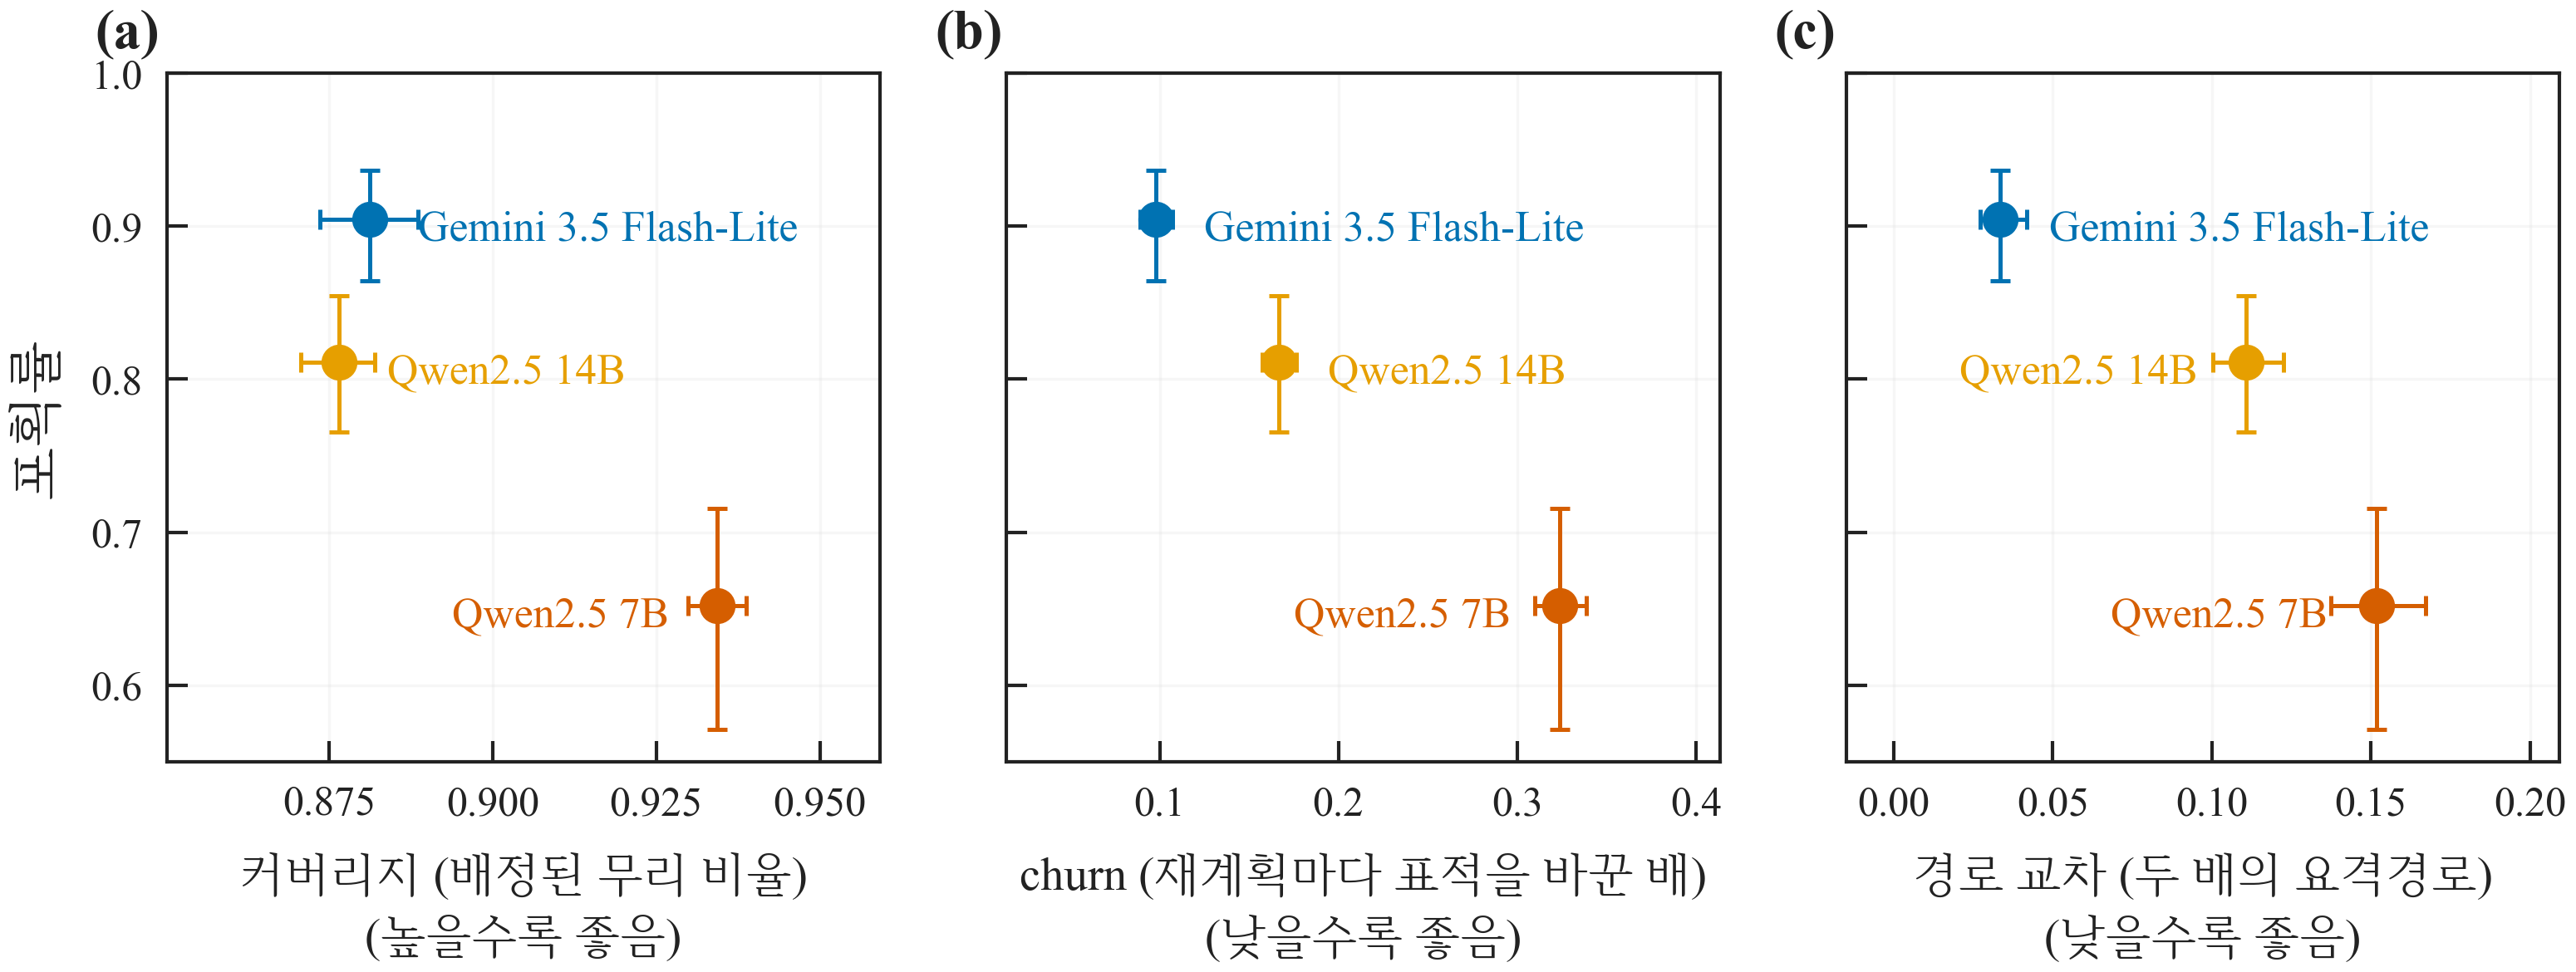
\includegraphics[width=\columnwidth]{fig18.png}
\caption{포메이션별·조건별 포획률(오차막대 95\,\% CI)}
\label{fig:condbars}
\end{figure}

\inputshortcap{지휘관 계획 품질과 성능}{tables/tab_planquality}

\subsection{제안 체계 전체}
\label{sec:res_g3}

\subsubsection{두 계층의 상호작용}
\label{sec:res_interaction}

식~\eqref{eq:interaction}의 상호작용을 9개 지표 전부에 대해 계산하였다(Table~\ref{tab:interaction}).

\inputshortcap{$2\times2$ 상호작용 분해(Gemini 지휘관)}{sections_kdu/tab_interaction_ell}

9개 지표 중 8개에서 상호작용이 유의하지 않고, 다중비교 보정 후에도 그대로 8개다. 두 계층의 기여는 상승이 아니라 가산적이다. 예외인 평균 포획 시각은
두 계층이 모두 제압을 앞당겨 생기는 수확체감이다. 가산성이 두 계층을 따로 써도 된다는 뜻은 아니다. 양동에서는 기동
계층 단독($-0.033$)도 전략 계층 단독($+0.070$)도 유의하지 않은데 결합은 $+0.090$ 으로
유의해진다. 무리 수와 방어정 수가 같아 배정과 기동이 둘 다 맞아야 막히기 때문이다.

\subsubsection{전 지표 효과크기}
\label{sec:res_effectsize}

제안 체계와 기준선의 차이를 9개 지표에 걸쳐 효과크기로 잰다(Table~\ref{tab:effectsize}).

\inputshortcap{전 지표 효과크기($|\dz|$ 내림차순)}{sections_kdu/tab_effectsize_ell}



개선은 기동 비용과 자원 효율에 몰려 있다. 총 선회량은 47\,\% 줄어 $\dz = -3.23$, 포획당
그물은 45\,\% 줄어 $-2.09$, 포획 이격거리는 $0.88\,\ell$ 늘어 $+1.81$ 인 반면 포획률은
$\dz = 0.44$ 로 최하위권이며, 다중비교 보정에서는 포획률만 유의성을 잃는다.
